\documentclass[paper=a4,oneside,fontsize=12pt, parskip=full]{scrartcl}
\usepackage{color,soul}
\usepackage[left=1.5cm,right=2.5cm,top=2cm,bottom=1.5cm]{geometry}
\usepackage{tikz-page}
\usepackage{framed}
\usepackage{bm}
\usepackage{tikz}
\usepackage{listings}
\usepackage{xcolor}
\usepackage{amsmath}

\definecolor{codegreen}{rgb}{0,0.6,0}
\definecolor{codegray}{rgb}{0.5,0.5,0.5}
\definecolor{codepurple}{rgb}{0.58,0,0.82}
\definecolor{backcolour}{rgb}{0.95,0.95,0.92}

\lstdefinestyle{mystyle}{
    backgroundcolor=\color{backcolour},
    commentstyle=\color{codegreen},
    keywordstyle=\color{magenta},
    numberstyle=\tiny\color{codegray},
    stringstyle=\color{codepurple},
    basicstyle=\ttfamily\footnotesize,
    breakatwhitespace=false,
    breaklines=true,
    captionpos=b,
    keepspaces=true,
    numbers=left,
    numbersep=5pt,
    showspaces=false,
    showstringspaces=false,
    showtabs=false,
    tabsize=2
}
\lstset{style=mystyle}

\begin{document}
    \section{The Integers}\label{sec:the-integers}
    The most common numbers are those used for counting, namely the numbers

    \[1,2,3,4,\dots\]

    which are called the \textbf{positive integers}.
    Even for counting, we need at least one other number, namely,

    \[0(zero)\]

    For instance, we may wish to count the number of right answers you may
    get on a test for this course, out of a possible 100.
    If you get 100, then all your answers were correct.
    If you get 0, then no answer was correct.
    The positive integers and zero can be represented geometrically on a line,
    in a manner similar to a ruler or a measuring stick:

    \begin{center}
        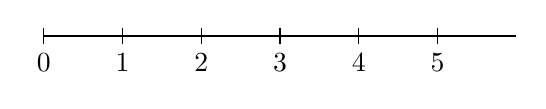
\begin{tikzpicture}
            % Draw the line
            \draw[thick] (0,0) -- (6,0);
            % Draw the ticks and labels
            \foreach \x in {0,1,2,3,4,5} {
                \draw (\x,0.1) -- (\x,-0.1) node[below] {\x};
            }
        \end{tikzpicture}
    \end{center}

    For this we first have to select a unit of distance, say the inch, and then on
    the line we mark off the inches to the right as in the picture.

    For convenience, it is useful to have a name for the positive integers
    together with zero, and we shall call these the \textbf{natural numbers}.
    Thus 0 is a natural number, so is 2, and so is 124,521.
    The natural numbers can be used to measure distances, as with the ruler.

    By definition, the point represented by 0 is called the origin.
    The natural numbers can also be used to measure other things.
    For example, a thermometer is like a ruler which measures temperature.
    However, the thermometer shows us that we encounter other types of numbers besides
    the natural numbers, because there may be temperatures which may go below 0.
    Thus we encounter naturally what we shall call \textbf{negative integers} which
    we call minus 1, minus 2, minus 3, \dots , and which we write as

    \[-1,-2,-3,-4,\dots\]

    We represent the negative integers on a line as being on the other side of 0
    from the positive integers, like this:

    \begin{center}
        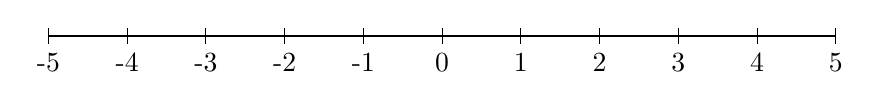
\begin{tikzpicture}
            % Draw the line
            \draw[thick] (-5,0) -- (5,0);
            % Draw the ticks and labels
            \foreach \x in {-5,-4,-3,-2,-1,0,1,2,3,4,5} {
                \draw (\x,0.1) -- (\x,-0.1) node[below] {\x};
            }
        \end{tikzpicture}
    \end{center}

    The positive integers, negative integers, and zero all together are called the integers.
    Thus $-9, 0, 10, -5$ are all integers.

    If we view the line as a thermometer, on which a unit of temperature has
    been selected, say the degree Fahrenheit, then each integer represents a certain temperature.
    The negative integers represent temperatures below zero.

    Our discussion is already typical of many discussions which will occur in
    this course, concerning mathematical objects and their applicability to physical situations.
    In the present instance, we have the integers as mathematical objects, which are essentially abstract quantities.
    We also have different applications for them, for instance measuring distance or temperatures.
    These are of course not the only applications.
    Namely, we can use the integers to measure time.
    We take the origin 0 to represent the year of the birth of Christ.
    Then the positive integers represent years after the birth of Christ (called AD years),
    while the negative integers can be used to represent BC years.
    With this convention, we can say that the year —500 is the year 500 BC .

    Adding a positive number, say 7, to another number, means that we must move 7 units to the right of the other number.
    For instance,

    \[5+7=12\]

    Seven units to the right of 5 yields 12.
    On the thermometer, we would of course be moving upward instead of right.
    For instance, if the temperature at a given time is 5° and if it goes up by 7°, then the new temperature is 12°.
    Observe the very simple rule for addition with 0, namely

    \noindent \textbf{N1.} \hspace{6cm} \fbox{
        \( 0 + a = a + 0 = a \)
    }

    for any integer \textbf{a}.

    What about adding negative numbers?
    Look at the thermometer again.
    Suppose the temperature at a given time is 10°, and the temperature drops by 15°.
    The new temperature is then -5°, and we can write

    \[10-15=-5\]

    Thus -5 is the result of subtracting 15 from 10, or of adding -15 to 10.
    In terms of points on a line, adding a negative number, say -3, to another
    number means that we must move 3 units to the left of this other number.
    For example,

    \[5+(-3)=2\]

    because starting with 5 and moving 3 units to the left yields 2.
    Similarly,

    \begin{center}
        7 + (-3 ) = 4, and 3 + ( -5 ) = -2 .
    \end{center}

    Note that we have

    \begin{center}
        3 + ( -3 ) = 0 or 5 + ( -5 ) = 0.
    \end{center}

    We can also write these equations in the form
    \begin{center}
    ( -3 )
        + 3 = 0 or ( -5 ) + 5 = 0
    \end{center}

    For instance, if we start 3 units to the left of 0 and move 3 units to the right, we get 0.
    Thus, in general, we have the formulas (by assumption):

    \noindent \textbf{N2.} \hspace{4cm} \fbox{
        \( a + (-a) = 0\) and \(-a + a = 0\)
    }

    In the representation of integers on the line, this means that \textbf{a} and \textbf{—a} lie
    on opposite sides of \textbf{0} on that line, as shown on the next picture:

    \begin{center}
        \begin{tikzpicture}
            % Draw the number line
            \draw[->] (-3,0) -- (3,0) node[right] {};

%            \draw (\x,0.1) -- (\x,-0.1) node[below] {\x};
            % Draw the points
            \draw (-2,0.1) -- (-2,-0.1) node[below] {$-a$} -- (-2,0.1);
            \draw (0,0.1) -- (0,-0.1) node[below] {$0$} -- (0,0.1);
            \draw (2,0.1) -- (2,-0.1)node[below] {$a$} -- (2,0.1);
        \end{tikzpicture}
    \end{center}

    Thus according to this representation we can now write

    \begin{center}
        3 = - ( -3 ) or 5 = - ( -5 ) .
    \end{center}

    In these special cases, the pictures are:

    \begin{center}
        \begin{tikzpicture}
            \draw[latex-latex] (-4.5,0) -- (4.5,0); % Axis
            \foreach \x in  {-3,-2,-1,0,1,2,3} % Vertical lines
            \draw[shift={(\x,0)},color=black] (0pt,3pt) -- (0pt,-3pt);
            \node at (-3,-0.5) {-3};
            \node at (0,-0.5) {0};
            \node at (3,-0.5) {3};
            \node at (4,-0.5) {$=-(-3)$};
        \end{tikzpicture}
    \end{center}


    \begin{center}
        \begin{tikzpicture}
            \draw[latex-latex] (-6.5,0) -- (6.5,0); % Axis
            \foreach \x in  {-5,-4,-3,-2,-1,0,1,2,3,4,5} % Vertical lines
            \draw[shift={(\x,0)},color=black] (0pt,3pt) -- (0pt,-3pt);
            \node at (-5,-0.5) {-5};
            \node at (0,-0.5) {0};
            \node at (5,-0.5) {5};
            \node at (6,-0.5) {$=-(-5)$};
        \end{tikzpicture}
    \end{center}

    \textbf{Remark:} We use the name minus \textbf{a} for \textbf{-a} rather than the words \textit{“negative a”}
    which have found some currency recently.
    I find the words \textit{“negative a”} confusing, because they suggest that \textbf{-a} is \textbf{a} negative number.
    This is not true unless \textbf{a} itself is positive.
    For instance,
    \[3 = -(-3)\]

    is a positive number, but 3 is equal to \textbf{-a}, where \textbf{a = -3}, and \textbf{a} is a negative number.

    Because of the property

    \[a + ( -a ) = 0\]

    one also calls \textbf{-a} the additive inverse of \textbf{a}.

    The sum and product of integers are also integers, and the next sections
    are devoted to a description of the rules governing addition and multiplication.
\end{document}